\documentclass[a4paper, 10pt]{article}        %\documentclass{} slides report proc book 
\usepackage[margin=1in]{geometry}
\usepackage[]{graphicx}
\usepackage{indentfirst}

\usepackage[hyperref]{xcolor}
\definecolor{teal}{RGB}{0, 128, 128}


\usepackage{hyperref, xcolor}
\hypersetup{
        colorlinks = true,
        allcolors={teal},
        linkcolor={teal}
       %urlcolor=[rgb]{0,128,128},
     }
%\title{Variants Statistics in Beacon}     
\title{Viral Beacon Variants statistics}  

\begin{document}
\date{}
\maketitle


\section{Summary Stats}


%Statistics are calculated using \href{https://github.com/clauw87/virusbeacon/blob/raw_ideas/query_by_region_alias.pdf}{\texttt{Query by region -by names/aliases}} and \href{https://github.com/clauw87/virusbeacon/blob/raw_ideas/filters.pdf}{\texttt{Filters}}.\\

%I would keep separate this by sequencing technology (platform): Illumina vs Nanopore (for now only Illumina) and of course fastq vs consensus (for now only fastq)

\begin{enumerate}

\item Number of variants in dataset: 
\item[] \textsl{by resource \& pipeline}:\\
SRA-Illumina: 45359, SRA-ONT: 28117, ENA: 5659, GISAID: 20288 
\item Number of genomic positions with variants: 28871/ Number of genomic positions: 29903 (96.15758\%)
\item[] \textsl{by resource \& pipeline}: \\
SRA-Illumina: 26366, SRA-ONT: 16304, ENA: 4833, GISAID: 13987 
\item Frequency of variants per position: fig \ref{fig:needle}
\item Number of variants per position: (3: 5769; 2: 11021; 1:11964) fig \ref{fig:needle}
% (also for Frequency (sampleMatchingCount), counts of unique sequences/haplotypes or counts of runs having them?)
   \begin{figure}[!htb]
     \centering
      \includegraphics[width=0.5\textwidth]{illum_needle.pdf}
            \includegraphics[width=0.5\textwidth]{ont_needle.pdf}
      \includegraphics[width=0.5\textwidth]{gbk_needle.pdf}
      \includegraphics[width=0.5\textwidth]{gisaid_needle.pdf}
       %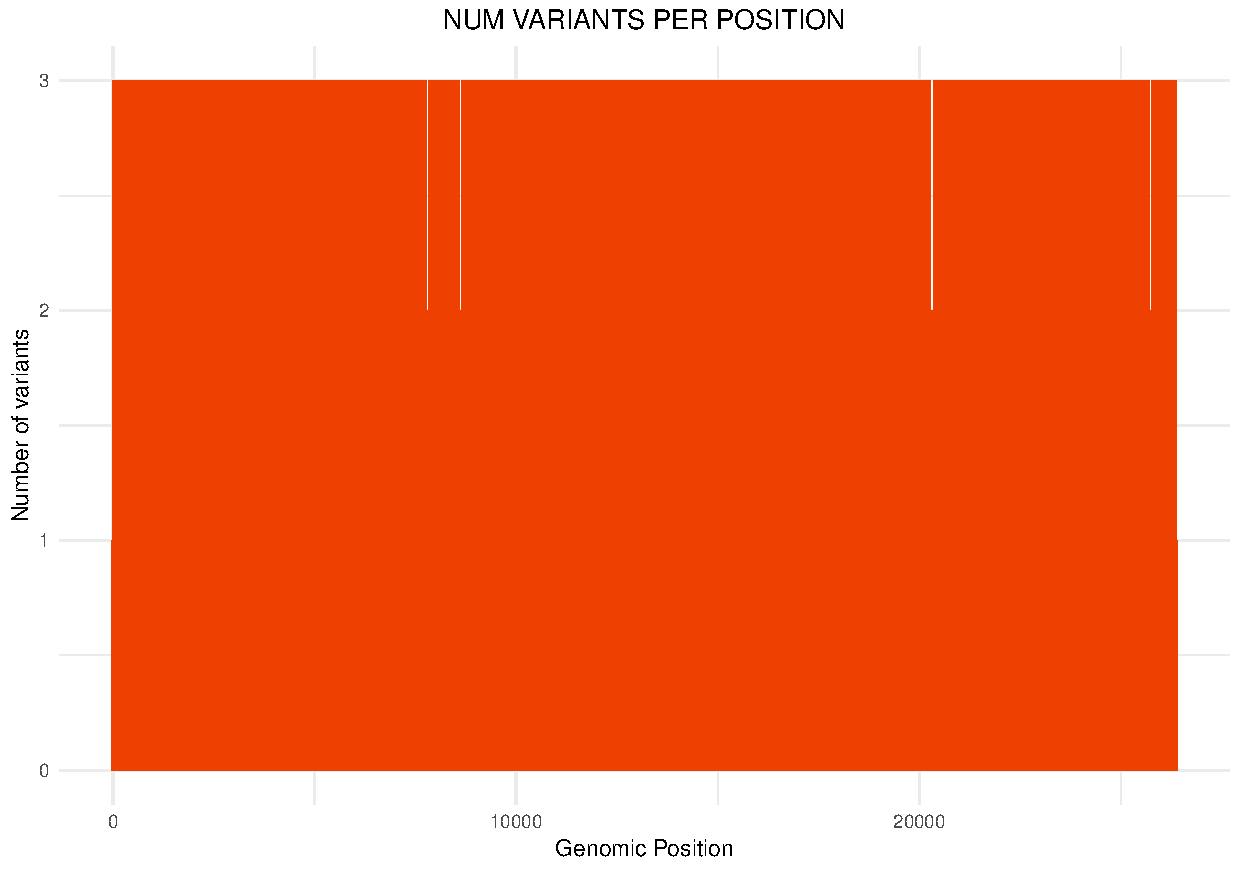
\includegraphics[width=0.8\textwidth]{needle_vpp.pdf}
       %\includegraphics[width=0.7\textwidth]{genome_line.pdf}
      %\includegraphics[width=0.8\textwidth]{stats_menu1.pdf}
      %\includegraphics[width=0.8\textwidth]{beacon_stats_gp.pdf}
      %\includegraphics[width=0.8\textwidth]{beacon_stats1.pdf}
     %\includegraphics[width=1.2\textwidth]{stats1.pdf}
    %\includegraphics[width=0.7\textwidth]{gral_stats.pdf}
    \caption{Needle plot: Frequency of variants per position per datasets}
     %\caption{Needle plot: Top: Frequency of variants per position. Bottom: Number of alternates per position}
     \label{fig:needle}
     \end{figure}
%\item[-] Unique Variant Frequency n terms of number of unique sequences/haplotypes having them/ sequences/haplotypes not having them\\
%\item[-] Variant Frequency in terms of number of runs having them/ runs not having them
\item Number of variants in database: 80860
\item[] \textsl{by resource \& pipeline}:\\


\begin{itemize}
%\item[\textsl{option}] Split by sequence database: SRA, GISIAD, GWH
%\item[\textsl{option}] Split by geographic region: Australia, China, USA, Singapur, etc
%\item[\textsl{option}] Split by collection date (month)
\item[\textsl{option}] Split by variant frequency (groups) fig \ref{fig:freq}
   
     \begin{figure}[!h]
     \centering
     \includegraphics[width=0.8\textwidth]{vars_per_fg_all.pdf}
      %\includegraphics[width=0.5\textwidth]{frequency.pdf} 
      %\includegraphics[width=1\textwidth]{by_protein.pdf}
  \caption{Number of variants per frequency group}
\label{fig:freq}
     \end{figure}
     
     
\item[\textsl{option}] Split by variant type field: SNP, MNP, INDEL, OTHER. fig \ref{fig:gral}
\item[\textsl{option}] Split by genomic region: coding: all with genomic region=CODING, non-coding: the rest fig (further UTRs, intergenic?) fig \ref{fig:gral}
%\item[\textsl{option}] Split by variant effect: SYNONYMOUS CODING/ NON SYNONYMOUS CODING/ STOP GAINED, NON-CODING/ INTERGENIC, etc
\item[\textsl{option}] Split by molecular consequence (grouped: SYN: SILENT, NON-SYN: MISSENSE+NONSENSE, NONCODING:the rest) and further in all classes as in fig \ref{fig:gral} 

     
%\item[\textsl{option}] Split by Biosample sample.type
%\item[\textsl{option}] Split by Individual sex
%\item[\textsl{option}] See Per region Statistics: Distribution in genomic regions: \underline{non-coding}, \underline{gene}, \underline{cds/mature peptide}, \underline{stem loops}. Number of variants aggregated in regions, show also split by syn/non syn,  as in fig \ref{fig:mp}.
\item[\textsl{option}] See Per region Statistics: Distribution in genomic regions. Upon click on genomic region graph, expand to see per number of variants distribution in genomic regions: select \underline{NON-CODING}, and within \underline{CODING} show options: \underline{gene}, \underline{cds/mature peptide}. This will show individual components of each class fig  \ref{fig:genes} and \ref{fig:mp}.

\end{itemize}
%\item Number of positions with aminoacid changes in database/ Number of coding positions
\item Number of variants producing unique aminoacid substitutions in database: 18308
\item[\textsl{option}] Filter upon \underline{cds/mature peptide}. Number of variants producing aminoacid changes are aggregated in mature protein region
\item Number of unique aminoacid changes per protein \ref{fig:aa}
\end{enumerate}

     
       

\section{Polymorphic sites}

\section{Intrahost variants}

\end{document}













